\Chapter{Fejlesztői dokumentáció}
\label{Chap:dokumen}

\Section{WordPress, mint a rendszer alapja}

A feladatot WordPress tartalomkezelő rendszer, illetve a most már szintúgy \href{https://automattic.com/}{Automattic} tulajdonában lévő \href{https://wordpress.org/plugins/woocommerce/}{WooCommerce} webáruház bővítmény segítségével valósítottam meg. Ezekre alapozva építettem meg egy kívánt és szükséges funkciókat tartalmazó plugint, valamint a weboldal megjelenését szolgáló sablont.

A  \href{https://wordpress.org/download/}{WordPress angol nyelvű alapcsomagjában} található Akismet és Hello Dolly kiegészítőket, valamint a Twenty Fourteen, Fifteen és Sixteen sablonokat (melyek egyébként a kiadás évét jelölik: 2014, 2015, 2016) eltávolítottam, a \href{https://hu.wordpress.org/}{magyar telepítőcsomagból} pedig áthelyeztem a nyelvi fájlokat tartalmazó \verb|/wp-content/languages| mappát a szükségtelen plugin és sablon nyelvi fájlok nélkül.

Ezt követően a \texttt{/wp-content/themes} mappában létrehoztam a saját fejlesztésű sablon mappáját \texttt{CCRMS-theme} néven, a \texttt{/wp-content/plugins} mappában pedig a \texttt{CCRMS-plugin} nevű mappát a tervezett bővítményhez.

Bővítmény esetében elegendő egy \verb|index.php| fájl egy minimális fejléccel és máris egy használható, bekapcsolható plugin lesz belőle, míg a sablon esetében az \verb|index.php| fájl mellett egy \verb|style.css| fájlra is szükség van, melynek fejlece szintúgy kötött.

A bővítmény fejlece (index.php):
\begin{lstlisting}
<?php
/*
Plugin Name: CCRMS Plugin
Plugin URI: http://users.iit.uni-miskolc.hu/~harkaly
Description: Content & Customer Relationship Management System plugin
Version: 2016.05.01.
Author: Harkály Gergő GOYLIZ
Author URI: http://users.iit.uni-miskolc.hu/~harkaly
Text Domain: ccrmsplugin
*/
\end{lstlisting}

A sablon stíluslapjának fejlece (style.css):

\begin{lstlisting}
/*
Theme Name: CCRMS Theme
Theme URI: http://users.iit.uni-miskolc.hu/~harkaly
Version: 2016.05.01.
Author: Harkály Gergő GOYLIZ
Author URI: http://users.iit.uni-miskolc.hu/~harkaly
Description: Content & Customer Relationship Management System WordPress Template
License: All rights reserved!
License URI: http://users.iit.uni-miskolc.hu/~harkaly
Tags: responsive
Text Domain: ccrmstemplate
*/
\end{lstlisting}

A \texttt{textdomain}-ről még a későbbiekben szó lesz, előljáróban annyit, hogy ez járul hozzá a sablon, illetve az egész honlap egyszerű többnyelvűsítéséhez.

\newpage

\Section{Biztonság}

A weboldal, illetve a rendszer biztonságosságát kritikus pontnak tekintettem, ennek érdekében igyekeztem mindent meg is tenni.

A WordPress adminisztrációs felülete a \texttt{/wp-login.php} vagy \texttt{/wp-admin} URL-eken érhető el, bár mindkét esetben valójában a \texttt{/wp-admin} mappa tartalma biztosítja a kezelőfelületet. Éppen ezért a \texttt{/wp-admin} mappát, így a belépési lehetőséget is egy \texttt{.htaccess}, \texttt{.htpasswd} párosítással korlátoztam le. Tehát a \texttt{wp-admin} mappában elhelyeztem egy \texttt{.htaccess} fájlt az alábbi kóddal:

\begin{lstlisting}
<Files admin-ajax.php>
	Order allow,deny
	Allow from all
	Satisfy any
</Files>

AuthName "admin + 1234"
AuthType Basic
AuthUserFile /path/to/.htpasswd
Require valid-user
\end{lstlisting}

A \texttt{wp-admin} mappában található \verb|admin-ajax.php| fájlra szüksége van több WordPress funkciónak is, ezért arról le kell venni a korlátozást, ezt  a kód első része biztosítja. Az \texttt{AuthName} által egyes böngészőkben meg is jelenik, hogy pontosan mit kell a felhasználónak beírni a felugró ablakba (admin, 1234), azonban ez kellő biztosítéknak bizonyult ahhoz, hogy megállítsa a robotokat, illetve az illetéktelen felhasználókat.

Az \texttt{AuthUserFile} értéke a \texttt{.htpasswd} fájl elérhetősége, melyben pedig az \verb|admin| felhasználónév és a hozzá tartozó \verb|1234| jelszó található az alábbi formában:

\begin{lstlisting}
admin:$apr1$La64E1Oj$USILkzSA3dshfT.L5nJ2B.
\end{lstlisting}

Ezen \texttt{.htpasswd} fájlt célszerű a webtárhely \texttt{public\_html} mappáján kívül elhelyezni, hogy HTTP/FTP kérésekkel se legyen elérhető.

Sikeres belépést követően megjelenik a WordPress bejelentkezési felülete, ahova alapesetben az egyedi felhasználónevet és a hozzátartozó jelszót szükséges megadni. Emellett bevezettem a catpcha beviteli mezőt is, ahol egyszerű matematikai feladatot, két egytől tízig random módon generált számot kell összeadnia a felhasználónak, egyéb esetben nem tud belépni.

A captcha kódja a Mellékletek > Forráskódok részben található meg. \ref{Chap:melleklet}

További biztonsági lépésként a bejelentkezési képernyőn alapértelmezetten megjelenő WordPress logót is eltüntettem egy stílusmódosítással:

\newpage

\begin{lstlisting}
// custom login
add_action('login_head', 'CustomLoginScreen');
function CustomLoginScreen()
{ ?>
	<style>
		body.login h1 { display:none; }
	</style>
<?php }
\end{lstlisting}

\begin{figure}
	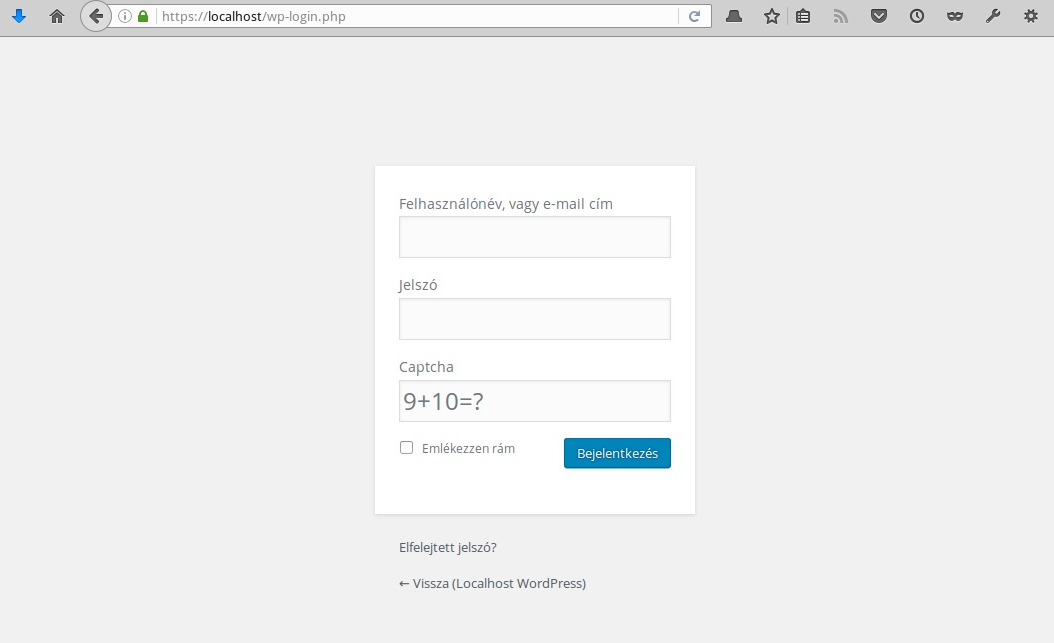
\includegraphics[width=1\textwidth]{wp-login-url.jpg}
	\caption{A bejelentkezési felület}
\end{figure}

A WordPress az adminisztrációs felületen feltöltött fájlokat alapértelmezetten a \texttt{/wp-content/uploads} mappába helyezi el, s bár alapvetően a Médiatárban feltölthető fájlok típusa korlátozva van, ettől még célszerű védekezni más típusú fájlok futtathatósága ellen. Ezért a jelölt mappában egy \texttt{.htaccess} fájlban az alábbi kódot helyeztem el, mely kizárólag a felsorolt kiterjesztésű fájlokat engedi olvasni:

\begin{lstlisting}
order deny,allow
deny from all
<files ~ ".(xml|css|jpe?g|png|gif|js)$">
	allow from all
</files>
\end{lstlisting}

A WordPress egy újabb kritikus pontja a felhasználónevek könnyű kinyerése, ugyanis az alap URL-hez társított \texttt{?author=[userID]} (itt a userID egy egész szám egytől kezdve, a meglévő felhasználók számáig bezárólag, lényegében a felhasználó adatbázis azonosítója) átirányít a felhasználó bejelentkezési nevéből (úgynevezett nickname) képzett URL-re (\texttt{/author/[username]}). Mivel a rendszer nyílt forráskódú, így a bejelentkezési felület elérhetősége mindenki (köztük hackerek) számára ismert, a felhasználónevek pedig így kinyerhetőek, ezért célszerű a WordPress ezen átirányítási funkcióját tiltani. Az erre szolgáló, bővítményben elhelyezett kód a következő, mely a \verb|?author=| kéréseket átirányítja a főoldalra:

\begin{lstlisting}
// redirects ?author= URLs to homepage to avoid getting author names
add_action('template_redirect', 'HideAuthorURL');
function HideAuthorURL()
{
	if (is_author())
	{
		wp_redirect(home_url());
		exit;
	}
}
\end{lstlisting}

A WordPress alapértelmezetten tartalmaz egy adminisztrációs felületről elérhető szerkesztőfelületet a bővítmények és sablonok fájljainak módosítására, azonban ez szintúgy biztonsági kockázatot jelent, ezért ezt letiltottam a \texttt{wp-config.php} fájlban elhelyezett alábbi kód segítségével:

\begin{lstlisting}
define('DISALLOW_FILE_EDIT', true);
\end{lstlisting}

A szintúgy ezen konfigurációs fájlban található \texttt{\$table\_prefix} változó értékét az eredeti \texttt{wp\_}-ról szintúgy megváltoztattam \texttt{ccrmswp\_}-re, hiszen a rendszer nyílt forráskódú mivolta miatt ez egy újabb biztonsági rés. Természetesen célszerű ennél bonyolultabb, randomgenerált prefixet használni.

A WordPress egy ingyenes, nemzetközi közösség által készített és folyamatosan továbbfejlesztett tartalomkezelő, ám az újítások nem kerülnek be automatikusan a rendszerbe, hanem SVN szerverekről tölthetőek le, akár csomagolt formátumban is. Ez egyik oldalról jó, hisz egy-egy bevezetett újítás vagy módosítás gondot okozhat egy korábban elkészített oldalnál, másrészt hátrány, hiszen így a szükséges (biztonsági) javítások sem települnek.

Ezért az alábbi kódokat a \texttt{wp-config.php} fájlban szintúgy célszerű elhelyezni, mely biztosítja az alaprendszer automatikus frissítését.

\begin{lstlisting}
// enable automatic update
define('WP_AUTO_UPDATE_CORE', true);
\end{lstlisting}

Emellett a harmadik fél által fejlesztett sablonok és bővítmények szintúgy SVN-ről tölthetőek le, melyek automatikus frissítése természetesen ugyanúgy ajánlott, melyet a pluginban elhelyezett alábbi kóddal biztosítok:

\begin{lstlisting}
// enable automatic updates for plugins
add_filter('auto_update_plugin', '__return_true');

// enable automatic updates for themes
add_filter('auto_update_theme', '__return_true');
\end{lstlisting}

A WordPress tartalomkezelővel készült honlapokat rengeteg támadás éri, hiszen lényegében rengeteg módszerrel leellenőrizhető automatikusan, hogy az adott weboldal motorja ismert CMS-e, ha igen, pontosan melyik az. Így például a \verb|wp-admin|, \verb|wp-login.php| fájlok megléte (200-as válaszüzenet a szervertől ezek lekérésekor), valamint a WP a website \texttt{<head>} részébe is elhelyez egy \texttt{<meta name="generator" content="WordPress" />} tagot. Ezt célszerű is eltávolítani, erre a WordPress szintúgy biztosít lehetőséget:

\begin{lstlisting}
// hide generator from header
remove_action('wp_head', 'wp_generator');
\end{lstlisting}

\Section{Többnyelvűsítés - iln18}

Az \texttt{iln18} egy nemzetközi jelzése a többnyelvűsítésnek, mely arra utal, hogy az \texttt{l} és \texttt{n} karakterek között nemzetközi viszonylatban összesen 18 másik karakter létezik. Bár a magyar nyelvben csak az \verb|ly| és \verb|m| foglal helyet, de nem feledkezhetünk meg más országok, népek nyelvéről sem.

A rendszer többnyelvűsítésére a WordPress-nél megismert PO/MO megoldást választottam, ahol a \texttt{.po} fájl a Portable Object, a \texttt{.mo} a Machine Object, azaz az elsőbe a fordítandó és a fordított szöveg kerül, míg a másodikba már gépi kódra fordított változat. Az fordítandó szövegek kiindulási állapotát egy \texttt{.pot} fájlba szokás összefoglalni. A PHP nyelvben ezen megoldás kezelésére a \texttt{gettext} függvénykönyvtár szolgál.

A \texttt{.po} tartalma kötelezően (természetesen az egyes megnevezések átírandóak):

\begin{lstlisting}
msgid ""
msgstr ""
"Project-Id-Version: CCRMS\n"
"Report-Msgid-Bugs-To: http://users.iit.uni-miskolc.hu/~harkaly/\n"
"POT-Creation-Date: 2016-01-30 01:00+0100\n"
"PO-Revision-Date: 2016-01-30 01:00+0100\n"
"Last-Translator: Harkály Gergő <harkaly@iit.uni-miskolc.hu>\n"
"Language-Team: Harkály Gergő <harkaly@iit.uni-miskolc.hu>\n"
"Language: hu\n"
"MIME-Version: 1.0\n"
"Content-Type: text/plain; charset=UTF-8\n"
"Content-Transfer-Encoding: 8bit\n"
\end{lstlisting}

Megjegyzéseket a \texttt{\#} jellel lehet elhelyezni, például a shell fordítási parancsot segítségképpen: \texttt{\#msgfmt textdomain-hu\_HU.po -o textdomain-hu\_HU.mo}

A fordítandó szövegeket a \texttt{msgid}, az adott nyelv megfelelőjét pedig a \texttt{msgstr} kulcsszavakkal kell meghatározni az alábbiakhoz hasonló formában:

\begin{lstlisting}
msgid "username"
msgstr "felhasználónév"

msgid "password"
msgstr "jelszó"
\end{lstlisting}

A két fájltípust egy \texttt{lang} (vagy languages) mappában célszerű elhelyezni, majd ezekre a fájlokra mind a sablonban (functions.php fájl), mind a bővítményben hivatkozni kell, melyre szintúgy van WordPress funkció:

\begin{lstlisting}
// load translated text for plugin
load_plugin_textdomain('ccrmsplugin', false, dirname(plugin_basename(__FILE__)).'/lang/');
// load translated text for theme
load_theme_textdomain('ccrmstheme', get_template_directory() . '/lang');
\end{lstlisting}

Fentebb látható is, hogy megjelent a korábban már említett \verb|textdomain|, melyet a fordítandó szövegek használatakor kell alkalmazni. A fordítási egységek megadásakor az első paraméter mindig a sablon vagy bővítmény \verb|textdomain| értéke, második pedig a fordítási fájlokat (.po, .mo) tartalmazó mappa elérési útvonala.

\Section{Saját fejlesztésű funkciók}

Bár a WordPress számos funkciót biztosít, melyekkel egy összetettebb honlapot is létre lehet hozni, mégis úgy gondoltam, a kódújrafelhasználás miatt célszerű néhány saját függvényt is definiálni.

Szerettem volna felkészülni a többnyelvűsítésre is, melyben a feltételezés az, hogy az egyes nyelvekhez tartozó oldalak URL-jében a fődomain mögött az adott nyelv két karakterből álló rövidített verziója fog majd szerepelni, például \texttt{domain.hu/en/}, \texttt{domain.hu/de/}. A megalkotott függvény segítségével először a link végének levágásával meghatározom az adott nyelvet, majd arra alapozva további konstans értékeket, hiszen a HTML tagok valamint különböző API-k \verb|lang| paramétere eltérhet (például hu-HU vagy hu\_HU). Nehezítette a dolgot, hogy az angol nyelv kétbetűs kódja egyértelműen az \texttt{en}, azonban például a \texttt{hu\_HU} és \texttt{de\_DE} meghatározáshoz hasonlóan nincs \texttt{en\_EN}, de van \texttt{GB} vagy \texttt{US}. Egyelőre a \texttt{GB} verzió mellett döntöttem.

\newpage

\begin{lstlisting}
// set locale variable based on URL substring
function SetLocaleByURL()
{
	$URLlang = substr(\$_SERVER['REQUEST_URI'], 1, 2);
	if($URLlang==='en')
	{
		$URLLANG = 'GB';
	}
	else
	{
		$URLLANG = strtoupper($URLlang);
	}
	define('locale', $URLlang);
	define('locale-LOCALE', $URLlang.'-'.$URLLANG);
	define('locale_LOCALE', $URLlang.'_'.$URLLANG);
	return;
}
\end{lstlisting}

Egy-egy oldal teljes URL-jének lekérése:

\begin{lstlisting}
// get current page full URL
function getFullURL()
{
	return 'http'.(isset($_SERVER['HTTPS']) ? 's' : '').'://'.$_SERVER['HTTP_HOST'].$_SERVER['REQUEST_URI'];
}
\end{lstlisting}

\Section{Sablon létrehozása}

A WordPress sablon számos fájlból épül fel a következők szerint:

\begin{itemize}
	\item 404.php - 404 hiba oldal sablonja
	\item archive.php - több speciális kategória sablonja, például a dátum szerinti rendezés esetében
	\item author.php - adott bejegyzést író adatlapjának sablonja
	\item category.php - kategóriák sablonja
	\item comments.php - hozzászólást biztosító űrlap és meglévő hozzászólások megjelenítésére szolgál, elhagyható
	\item footer.php - lábléc sablonja
	\item functions.php - mind a külső, mind a belső (admin panel) funkciók megadására szolgál, elhagyható
	\item header.php - a sablon fejlecének kódjait tartalmazza
	\item index.php - kezdőoldal beállítása
	\item page.php - Oldal sablonminta
	\item page\_egyedi.php - egyedi Oldal sablonminta is alkotható
	\item screenshot.png - admin panelben a választható sablonoknál megjelenő kép
	\item search.php - keresési eredmények megjelenítésére szolgál, elhagyható
	\item sidebar.php - oldalsáv sablonminta
	\item single.php - Bejegyzés sablonminta
	\item style.css - legfőképpen a sablon adatait tartalmazza
	\item tag.php - címke sablonminta
\end{itemize}

A sablon optimális működéséhez számos funkciót kell deklarálni annak mappájában (\texttt{/wp-content/themes/CCRMS-theme}) található \texttt{functions.php} fájlban.

Ahhoz, hogy a bejegyzésnél legyen lehetőség kapcsolódó, kiemelt kép feltöltésére, illetve annak a weboldalon történő megjelenítésére, az alábbi kódot kell elhelyezni a fent jelölt funkciókat tartalmazó fájlban:

\begin{lstlisting}
// add theme post thumbnail support
add_theme_support('post-thumbnails');
\end{lstlisting}

2016-ban értelmetlennek tűnik olyan honlapot készíteni, amely nincs felkészítve a közösségi oldalakra, így az ehhez szükséges metaadatokat is beépítettem a sablonba. A \href{https://developers.facebook.com/docs/sharing/webmasters}{Facebook Open Graph}-ra alapozva, a WordPress függvényeit kihasználva helyeztem el a sablon \texttt{header.php} fájljában azt a kódot, mely a mellékletben megtalálható. \ref{Chap:melleklet}

A \href{https://dev.twitter.com/cards/overview}{Twitter Cards} hasonló elven működik, a kapcsolódó meta tagokat szintúgy a \texttt{header.php}-ban kell elhelyezni:

\begin{lstlisting}
	<!-- Twitter Cards | https://dev.twitter.com/cards/overview -->
	<meta name="twitter:card" content="summary" />
	<meta name="twitter:site" content="@" />
	<meta name="twitter:title" content="<?php wp_title(''); ?>" />
	<meta name="twitter:description" content="<?php if(is_home()) { bloginfo('description'); } else { getPostExcerptOutsideLoop($post->ID, 160, FALSE); } ?>" />
	<meta name="twitter:image" content="<?php if(has_post_thumbnail($post->ID)) echo wp_get_attachment_image_src(get_post_thumbnail_id($post->ID), 'medium')['0']; ?>" />
\end{lstlisting}

A Pinterestnél csupán egyetlen sor szükséges a weboldal igazolásához:

\begin{lstlisting}
	<!-- Pinterest domain verify -->
	<meta name="p:domain_verify" content="<?=get_theme_mod('pinterestDomainVerifyID');?>">
\end{lstlisting}

A Google keresőoptimalizálást segítő egyik eszköze a \href{https://www.google.com/webmasters/tools/home?hl=HU}{Search Console}, a hozzá tartozó információk meta tagja:

\begin{lstlisting}
	<!-- Google Search Console -->
	<meta name="google-site-verification" content="">
\end{lstlisting}

\Section{A Bootstrap bemutatása}

Manapság elengedhetetlen a reszponzív megjelenés, azaz ahogy azt mondani szokták: kijelzőfüggetlen megjelenés, bár én pont hogy kijelzőfüggőnek nevezném. Mitöbb, a \href{https://webmasters.googleblog.com/2015/02/finding-more-mobile-friendly-search.html}{Google rangsorolási algoritmusának része lett 2015. április 21-től}, így a mobilos keresések során azok a weboldalak, melyek nincsenek felkészítve a kisebb kijelzőméretekre, hátrányos megkülönböztetésben részesülnek. (Itt megjegyezném, hogy 2016-ra még ennél is komolyabb változásokat helyeztek kilátásba a legnagyobb technológia cégek az \href{https://www.ampproject.org/}{Accelerated Mobile Pages Project} keretében, hogy még jobban növelni tudják a mobilos felhasználói élményt.)

A kijelzőfüggetlen megjelenés kialakításához a \href{http://getbootstrap.com/}{Boostrap}et választottam. A Bootstrap a legnépszerűbb HTML, CSS és JS keretrendszer reszponzív, úgynevezett ``mobile first'' projektek megalkotásához. A mobile first kifejezés egy szemléletmód, mely arra utal, hogy a projekt megvalósítása során a mobilos megjelenés kerül előtérbe, s nem a teljes képernyőre helyeződik a fókusz, ezért igyekszik minimalizálni a szükséges kódokat, hiszen egy mobiltelefon nyilván kisebb memória és processzor kapacitással rendelkezik, nem beszélve a mobilnet sebességéről.

A Bootstrap egy sort 12 oszlopra oszt fel (col-*-*), s ezeket a részeket tehetjük egymás mellé, alá. Emellett négy méretben gondolkodik, melyeket az \verb|xs, sm, md, lg| kulcsszavak jelölnek, tehát egy egység oszlopainak száma akár a mobil, tablet, PC függvényében deklarálhatóak, például: \texttt{col-sm-12}, \texttt{col-md-8}, \texttt{col-lg-4}.

Mivel a WordPress alapvetően nem Bootstrapre építkezik a sablonok esetében, így szükség volt a menüsáv kialakításánál egy már kész komponens használatára: \url{https://github.com/twittem/wp-bootstrap-navwalker}

\newpage

\Section{Felhasználói elégedettség növelése}

\SubSection{Keresőmező}

A WordPress-nek van beépített funkciója a Bejegyzésekhez/Oldalakhoz való hozzászólásra, ám a kéretlen kommentek (spam) elkerülése végett célszerű ezt regisztrációhoz kötni. Tekintettel arra, hogy a Facebook jelentősen az emberek életévé vált, ezért integráltam a \href{https://developers.facebook.com/docs/plugins/comments/}{Facebook Comments Plugin}t. Emellett egy másik szolgáltatás is egyre nagyobb teret nyer az online világban a hozzászólások esetében, mégpedig a \href{https://disqus.com/}{Disqus}. A bejegyzések alatt megjelenő hozzászólási lehetőségnél tehát három opció megjelenik a következő sorrendben: Disqus, Facebook, (WordPress) fiókkal rendelkezőknek.

\begin{figure}
	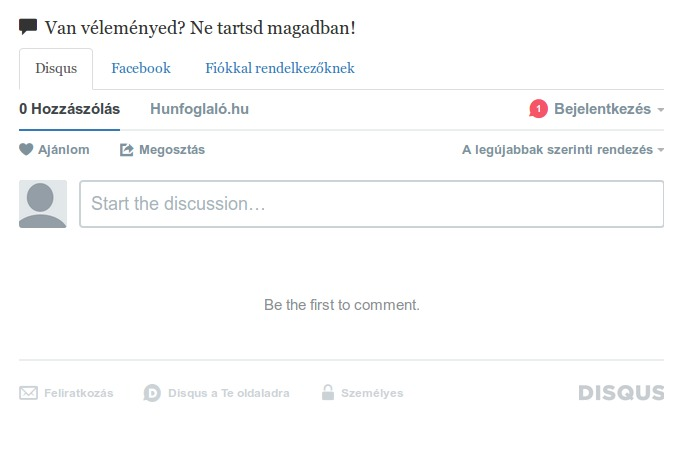
\includegraphics[width=1\textwidth]{comment-block.jpg}
	\caption{Hozzászólási lehetőség a bejegyzések alatt}
\end{figure}

\SubSection{Marketing}

\tab\textbf{CTO gomb}

CTO, azaz call-to-action gomb, mely azonnali cselekvésre ösztönöz, ennek cél linkje, valamint a felirata tetszőlegesen módosítható (például Hívjon most!, Kérjen útirányt a bolthoz!, Vásároljon most!).

\newpage

\textbf{Megosztógombok}

Napjainkban az online marketing elkerülhetetlen eleme a közösségi oldalak kihasználása, lényegében a weboldal felhasználóinak segítségével költségmentesen juthat el új személyekhez egy-egy tartalom, legyen az blogbejegyzés, vagy egy webshop terméke. Ezért automatikusan megjelentetek négy gombot a bejegyzések végén népszerűségi sorrendben: Facebook, Twitter, Google Plus és Nyomtatás. A Facebooknál a Facebook API segítségével azt is lekérdezem, hogy az adott bejegyzést hányszor osztották meg összesen.

\begin{lstlisting}
// display share buttons after posts
function ShareButtons()
{
	// Facebook stat number
	$FacebookJSON = json_decode( file_get_contents( 'https://api.facebook.com/method/links.getStats?urls=' . getFullURL().'&format=json' ), true);
	?>
	<div class="row text-center">
		<p style="text-align:center;"><i>Ha szerinted másokat is érdekelhet ez a cikk, akkor oszd meg velük!</i></p>
		<a target="_blank" rel="nofollow" href="https://www.facebook.com/sharer/sharer.php?u=<?php the_permalink() ?>" class="btn btn-primary btn-xs"><span class="glyphicon glyphicon-share-alt"></span> <span class="hidden-xs">Megosztás Facebookon (<?=$FacebookJSON['0']['total_count'];?>)</span></a>
		<a target="_blank" rel="nofollow" href="https://twitter.com/home?status=<?php the_permalink() ?>" class="btn btn-info btn-xs"><span class="glyphicon glyphicon-share-alt"></span> <span class="hidden-xs">Megosztás Twitteren</span></a>
		<a target="_blank" rel="nofollow" href="https://plus.google.com/share?url=<?php the_permalink() ?>" class="btn btn-danger btn-xs"><span class="glyphicon glyphicon-share-alt"></span> <span class="hidden-xs">Megosztás Google Plus-on</span></a>
		<a onclick="window.print();" class="btn btn-default btn-xs"><span class="glyphicon glyphicon-print"></span> <span class="hidden-xs">Nyomtatás</span></a>
	</div>
<?php }

\end{lstlisting}

\begin{figure}
	
\includegraphics[width=1\textwidth]{share-buttons.png}
	\caption{Megosztogombok a bejegyzések végén}
\end{figure}